\chapter{The Nature of Mathematical Inquiry}\label{chapter:induction}

\section{Brief Remarks on the History of Number Theory}

\subsection{The Ancient Greek Scholars}

\begin{figure}[p]
  \centering
  \begin{tikzpicture}
    \node[inner sep=0pt, rounded corners=0.5em, clip] {%
      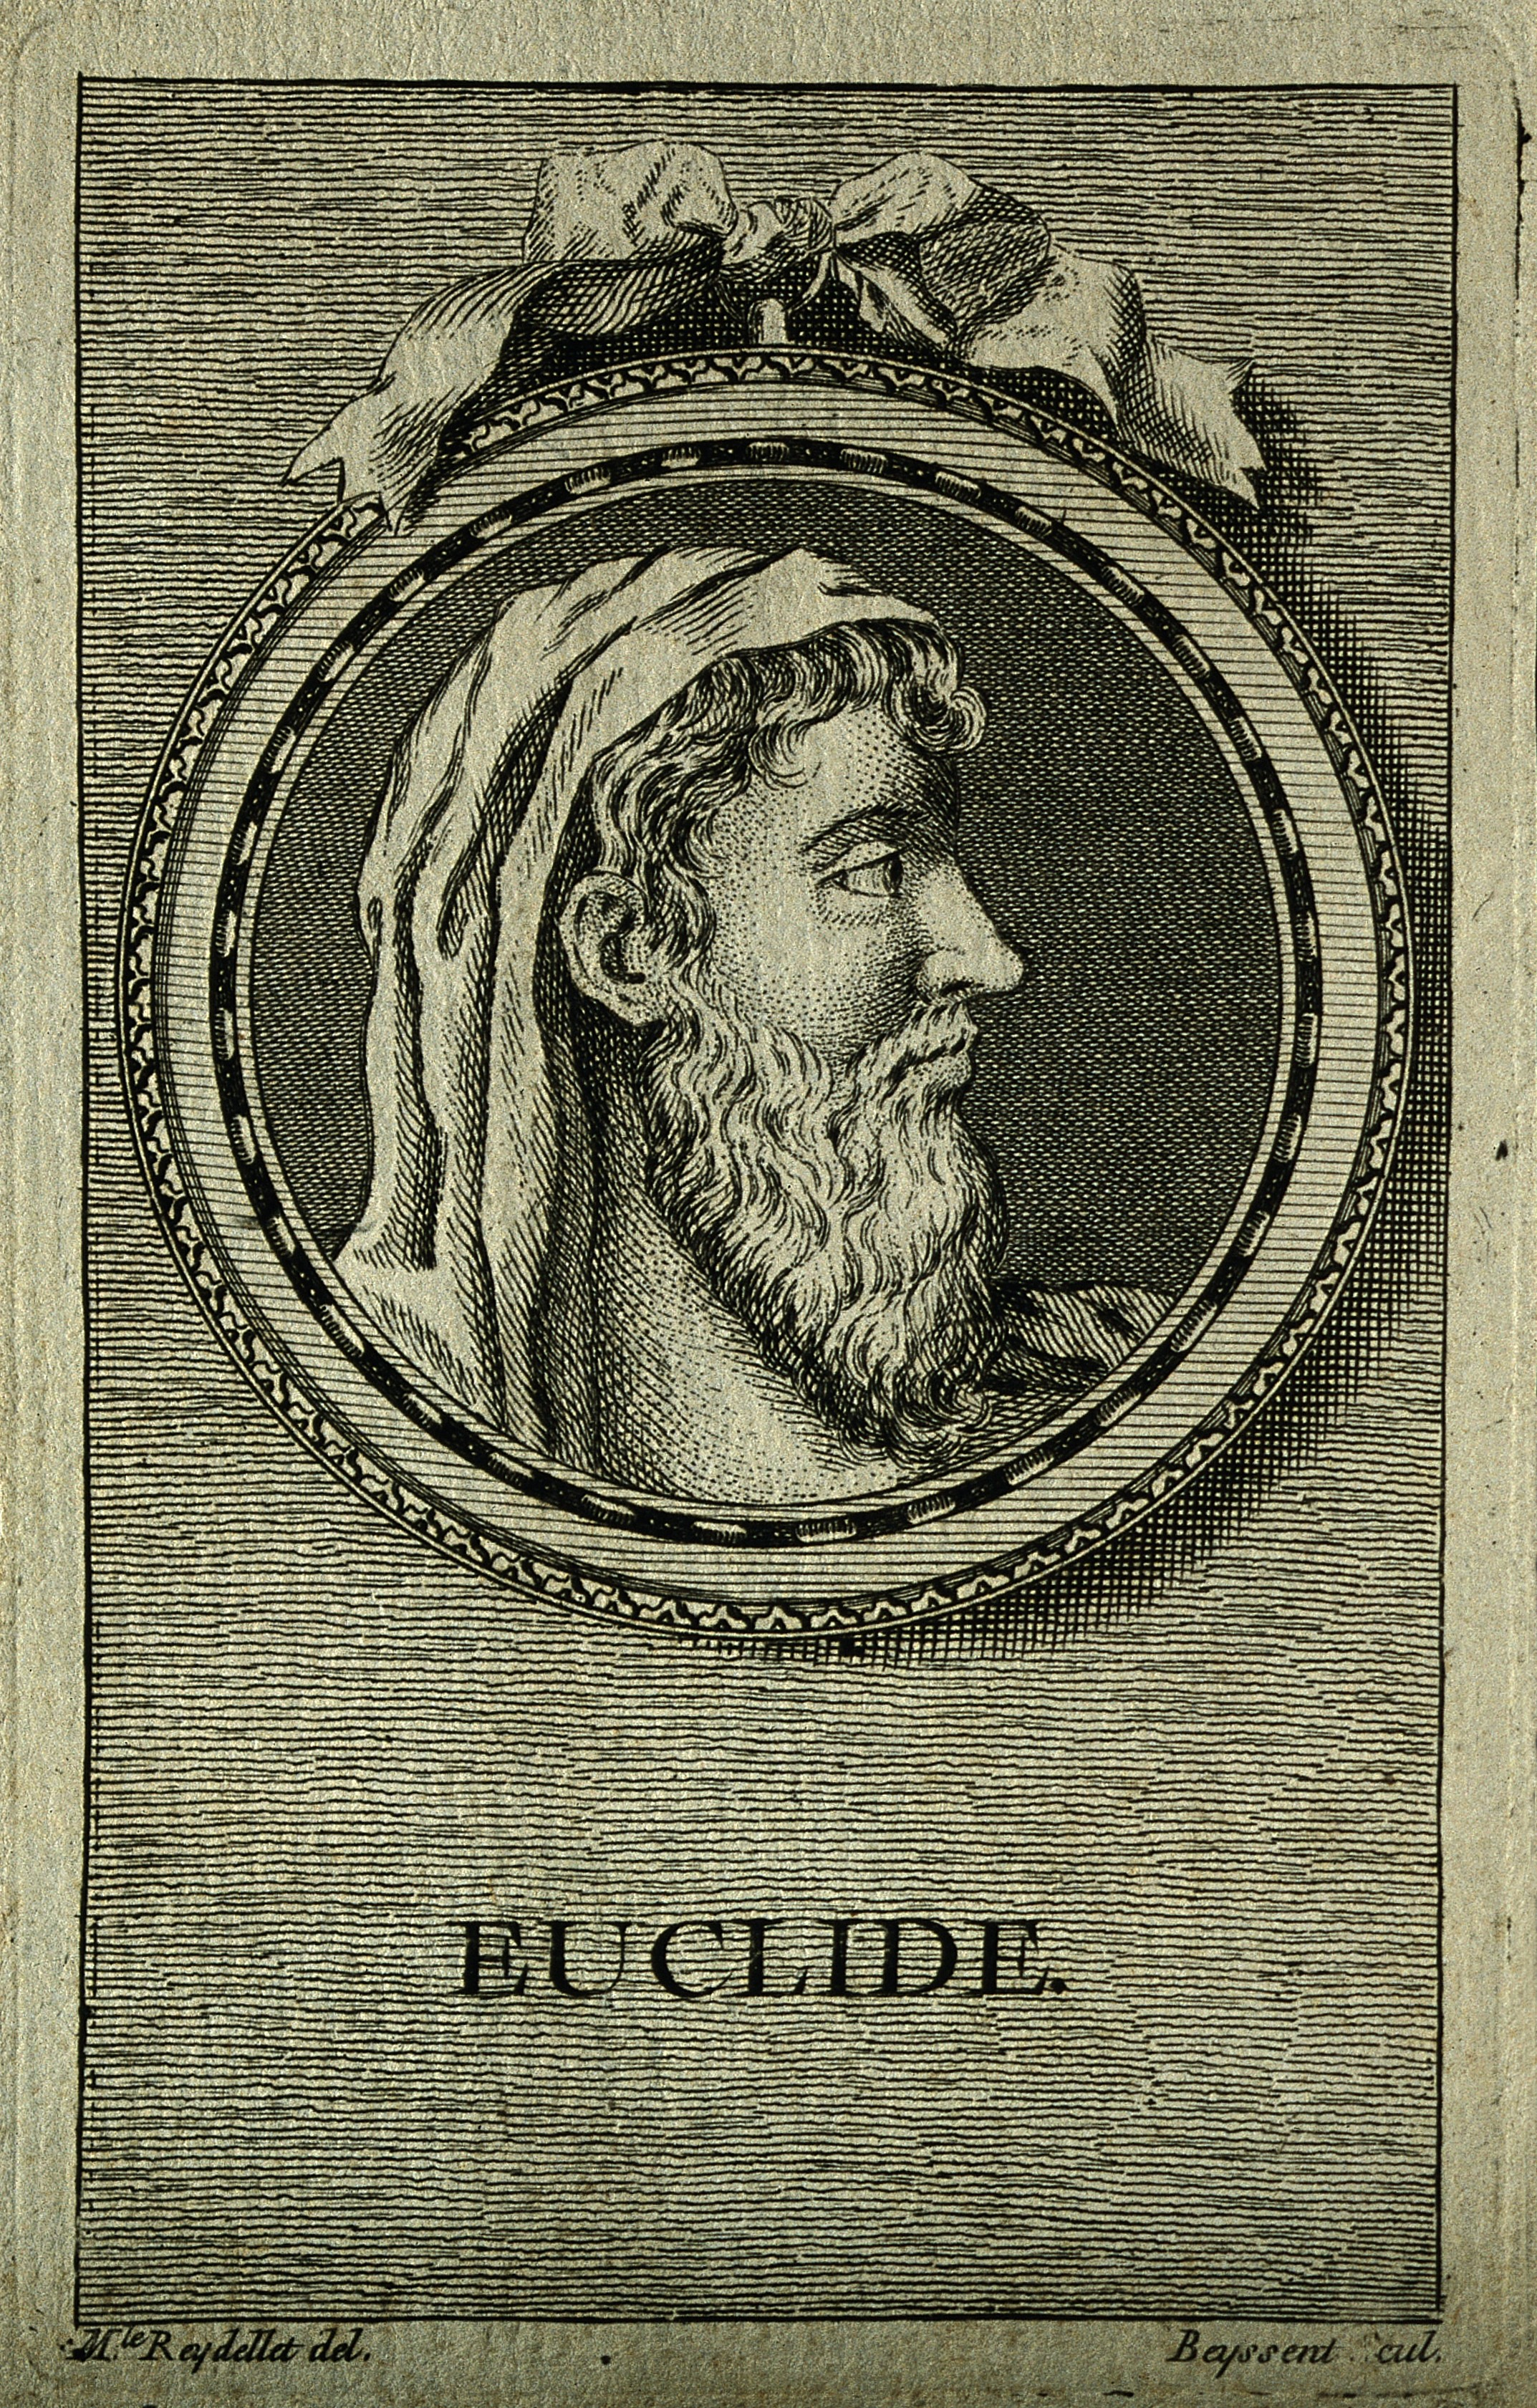
\includegraphics[
        alt={Portrait of Euclid of Alexandria.},
        height=\dimexpr.95\textheight-2pt\relax
      ]
      {figures/Euclid-Beyssent-line-engraving.jpg}%
    };
  \end{tikzpicture}
  \caption[Euclid of Alexandria]{\sloppy{Euclid of Alexandria. Line engraving by S. Beyssent after Mlle. C. Reydell.}}
  \label{figure:euclid}
\end{figure}

Number theory has a long history that dates back to antiquity. While a more complete history of mathematics would include findings about earlier civilizations \cite{boyer2011}, we begin our story in the Hellenistic city of Alexandria, which was founded by Alexander the Great in 331 BCE on the Mediterranean coast of Egypt. After the death of Alexander the Great in 323 BCE, Egypt came under the control of his general Ptolemy, who first ruled as satrap and became king of Egypt in 305/304 BCE \cite{fraser1972,holbl2001}. During the early Ptolemaic period, the city of Alexandria saw great development, such as the founding of the Mouseion, a state-supported research and teaching institution in which also the Library of Alexandria was housed \cite{casson2001}. This is the intellectual milieu in which Euclid of Alexandria likely lived, taught, and wrote one of the most influential manuscripts in the history of mathematics, the \textsc{Elements} \cite{euclid2015,heath1981}. In this monumental work, which is conventionally dated to around 300 BCE, Euclid systematically derived several key results in geometry and number theory from a small number of postulates. These include the infinitude of primes and the algorithm for finding the greatest common divisor, which bears his name. The 5\supth-century mathematical commentator Proclus reports in his commentary on Euclid's Elements that king Ptolemy came to Euclid with the question whether there is a quicker way of learning geometry \cite{proclus1992}. We can easily imagine the king recognizing the importance of Euclid's axiomatic approach but struggling with Euclid's careful derivations, and surely his royalty should not have to work through all thirteen books of the \textsc{Elements}. To which Euclid replied with the famous apothegm: \emph{"There are no royal roads to geometry."}

Around 250 CE, the Greek mathematician Diophantus of Alexandria wrote his \textsc{Arithmetica} \cite{diophantus1910}, which focused on solving equations with integer coefficients in one or multiple unknowns. This 13-volume work is often considered the first comprehensive treatment of algebra, though Diophantus relied on rhetorical descriptions rather than modern algebraic notation. Only six of the original volumes have survived, but they profoundly influenced later mathematicians.

The works of Euclid and Diophantus were preserved and studied by scholars in the Byzantine Empire, such as Theon of Alexandria and his daughter Hypatia. They added commentaries that clarified and expanded upon the original text.

During the Islamic Golden Age, scholars like Al-Khwarizmi, Ibn al-Haytham, and Omar Khayyam preserved and expanded upon the works of Euclid and Diophantus. Al-Khwarizmi's work, especially his \textsc{Kitab al-Mukhtasar fi Hisab al-Jabr wal-Muqabala} (from which the term "algebra" originates), introduced systematic methods for solving linear and quadratic equations. He used rhetorical algebra, like Diophantus, but began a transition toward symbolic representation by relying on consistent terminology for operations and equations.

After the invention of the printing press, Erhard Ratdolt, a German printer based in Venice, produced the first printed edition of the \textsc{Elements} in 1482. This edition included mathematical diagrams and marked an important step in the dissemination of Euclid's work. The first printed edition of Diophantus' \textsc{Arithmetica} was published in 1575 by Wilhelm Xylander, a German mathematician. The printing was done in Basel, Switzerland, which was a major hub for academic publishing at the time. By the time of Pierre de Fermat in the 17\supth{} century, both the \textsc{Elements} and \textsc{Arithmetica} had become essential texts for mathematicians across Europe, influencing the development of number theory and inspiring Fermat’s pioneering discoveries.

\subsection{Mathematics, Astronomy, and Poetry in Ancient India}

We could not move forward with the story of the greatest mathematical achievements without first turning our attention to the scholarly traditions of ancient India.

\subsection{Pierre de Fermat}

\begin{figure}[p]
  \centering
  \begin{tikzpicture}
    \node[inner sep=0pt, rounded corners=0.5em, clip] {%
      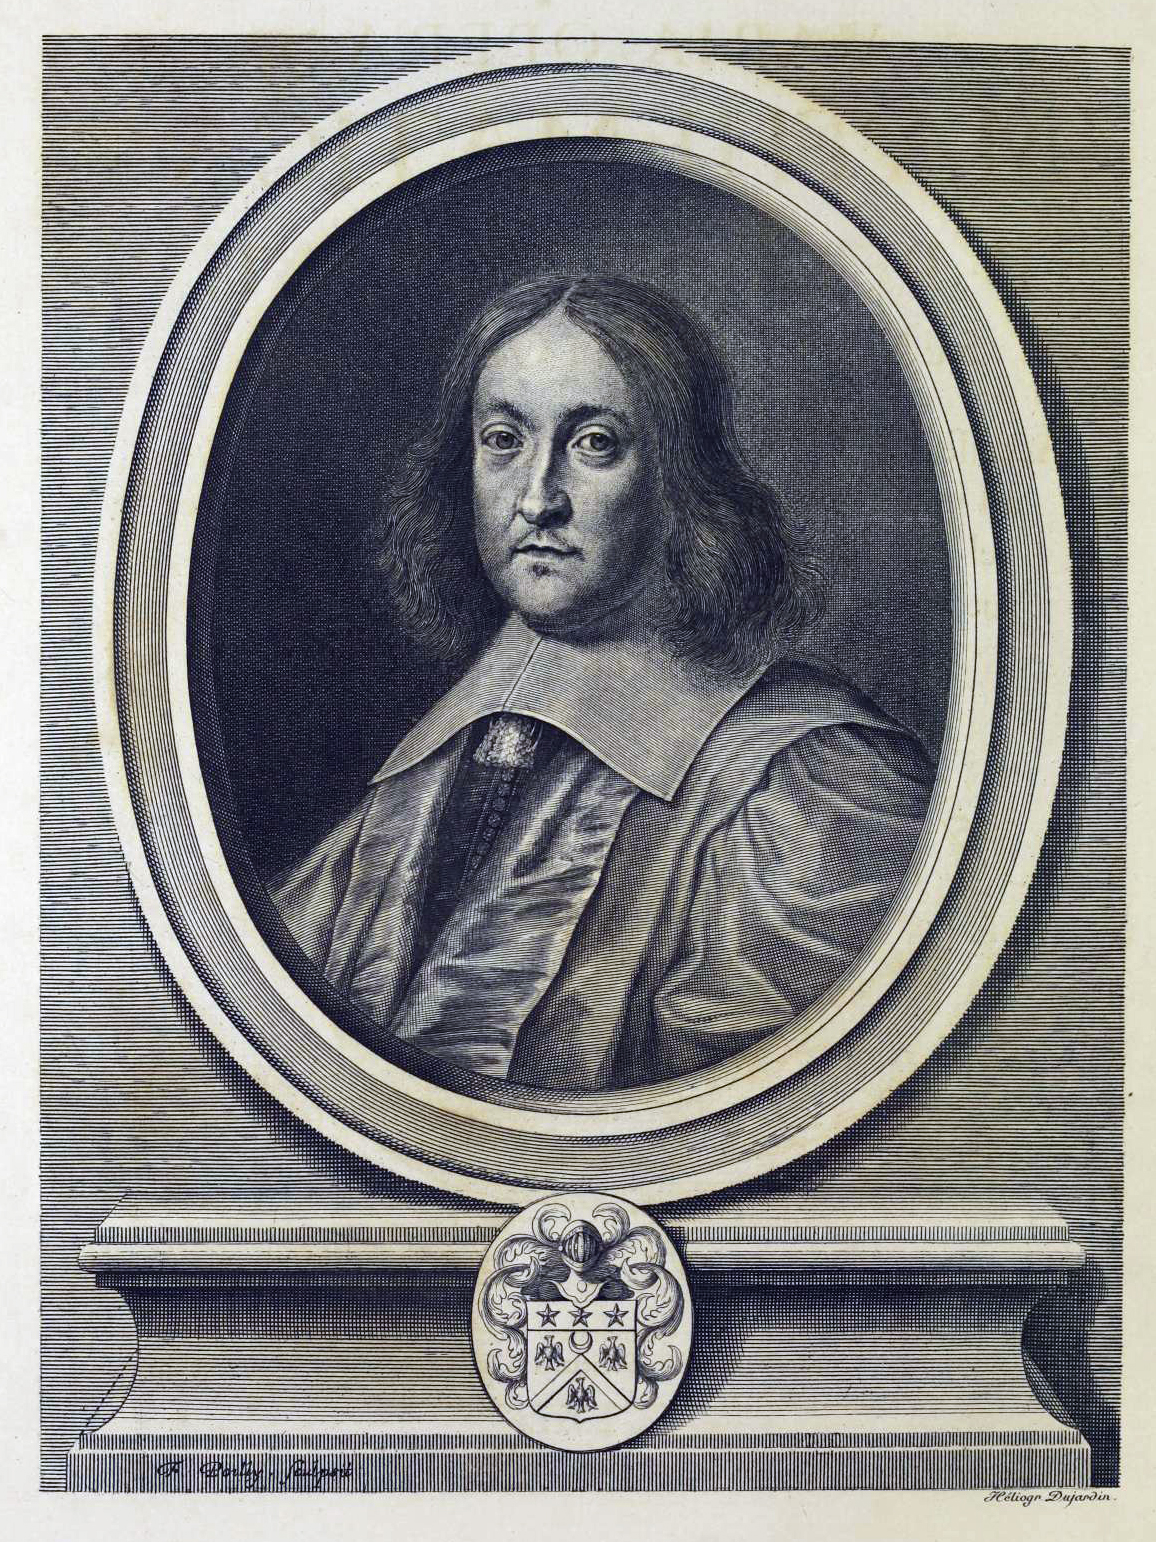
\includegraphics[
        alt={Portret of Pierre de Fermat.},
        height=\dimexpr.95\textheight-2pt\relax
      ]{figures/Fermat.jpg}%
    };
    \end{tikzpicture}
    \caption[Pierre de Fermat]{Pierre de Fermat. Engraving in Oeuvres Mathématiques Diverses.}
  \label{figure:fermat}
\end{figure}

Pierre de Fermat (1607--1665) is often considered the founder of modern number theory \cite{mahoney1994,weil1984}. He was a contemporary of Blaise Pascal and Marin Mersenne, both of whom he corresponded with, and also of Galileo Galilei. He wrote a manuscript titled \textsc{Éléments de Géométrie}, which served as an extension and commentary on Euclid’s \textsc{Elements}. In this work, he sought to modernize Euclid’s geometry by applying the emerging methods of algebra and analytic geometry to classical geometric problems.

Fermat made many groundbreaking discoveries in the theory of numbers. Among his most influential discoveries is \emph{Fermat's Little Theorem}, which states that if $p$ is a prime number, then
\begin{equation*}
  a^p\equiv a\pmod{p}.  
\end{equation*}
This theorem is key to many further results in modular arithmetic, and has modern applications in RSA encryption. Fermat also came up with the method of \emph{infinite descent}, which allows one to show that a certain equation or proposition cannot hold by showing that it would lead to an infinite descending sequence of positive integers. Fermat was very fond of this method, and used it brilliantly to prove some of his most profound claims. For instance, the case $n=4$ of \emph{Fermat's Last Theorem}, which states that there are no positive integers $x$, $y$, and $z$ such that $x^4+y^4=z^4$ is proven using infinite descent. In order to prove this fact, Fermat also showed that the area of a Pythagorean triangle is never a perfect square. Fermat is furthermore famous for the \emph{Two-Squares Theorem}, which states that any prime $p\equiv 1\pmod{4}$ can be written uniquely as a sum of two squares, and that primes $p\equiv 3\pmod{4}$ cannot be written as a sum of two squares. Fermat also claimed that any number can be written as the sum of at most three triangular numbers, as the sum of four squares, as the sum of five pentagonal numbers, and so on, but he did not indicate how these claims might be proven. The case of the triangular numbers is now known as Gauss's \emph{Eureka Theorem}, the \emph{Four-Squares} theorem was proven by Lagrange, and Cauchy proved the general theorem asserting that any number can be expressed as the sum of at most $n$ $n$-gonal numbers.

Fermat also made several famous conjectures. He conjectured that the equation $x^2+Ny^2=1$ has infinitely many solutions for any non-square integer $N$. Euler made a significant advance to this problem by proving it for specific values of $N$. The general form of the solution to equations of the form $x^2+Ny^2=1$ was found later by Legendre and Lagrange.

Finally, Fermat famously asserted that there could be no three positive integers $x$, $y$, and $z$ such that the equation
\begin{equation*}
  x^n+y^n=z^n
\end{equation*}
holds, when $n\geq 3$. This statement is now known as \emph{Fermat's Last Theorem}. He claimed to have a "truly marvelous proof", but that the margin of his copy of \textsc{Arithmetica} was too small to contain it. His assertion, known as \emph{Fermat's Last Theorem}, captivated mathematicians for centuries. It was finally proven in 1995 by Andrew Wiles, about 350 years after Fermat made his famous note in the margin, using advanced techniques from algebraic geometry and modular forms. Wiles’s achievement is considered one of the most remarkable milestones in the history of mathematics.

\subsection{Leonhard Euler}

\begin{figure}[p]
  \centering
  \begin{tikzpicture}
    \node[inner sep=0pt, rounded corners=0.5em, clip] {%
      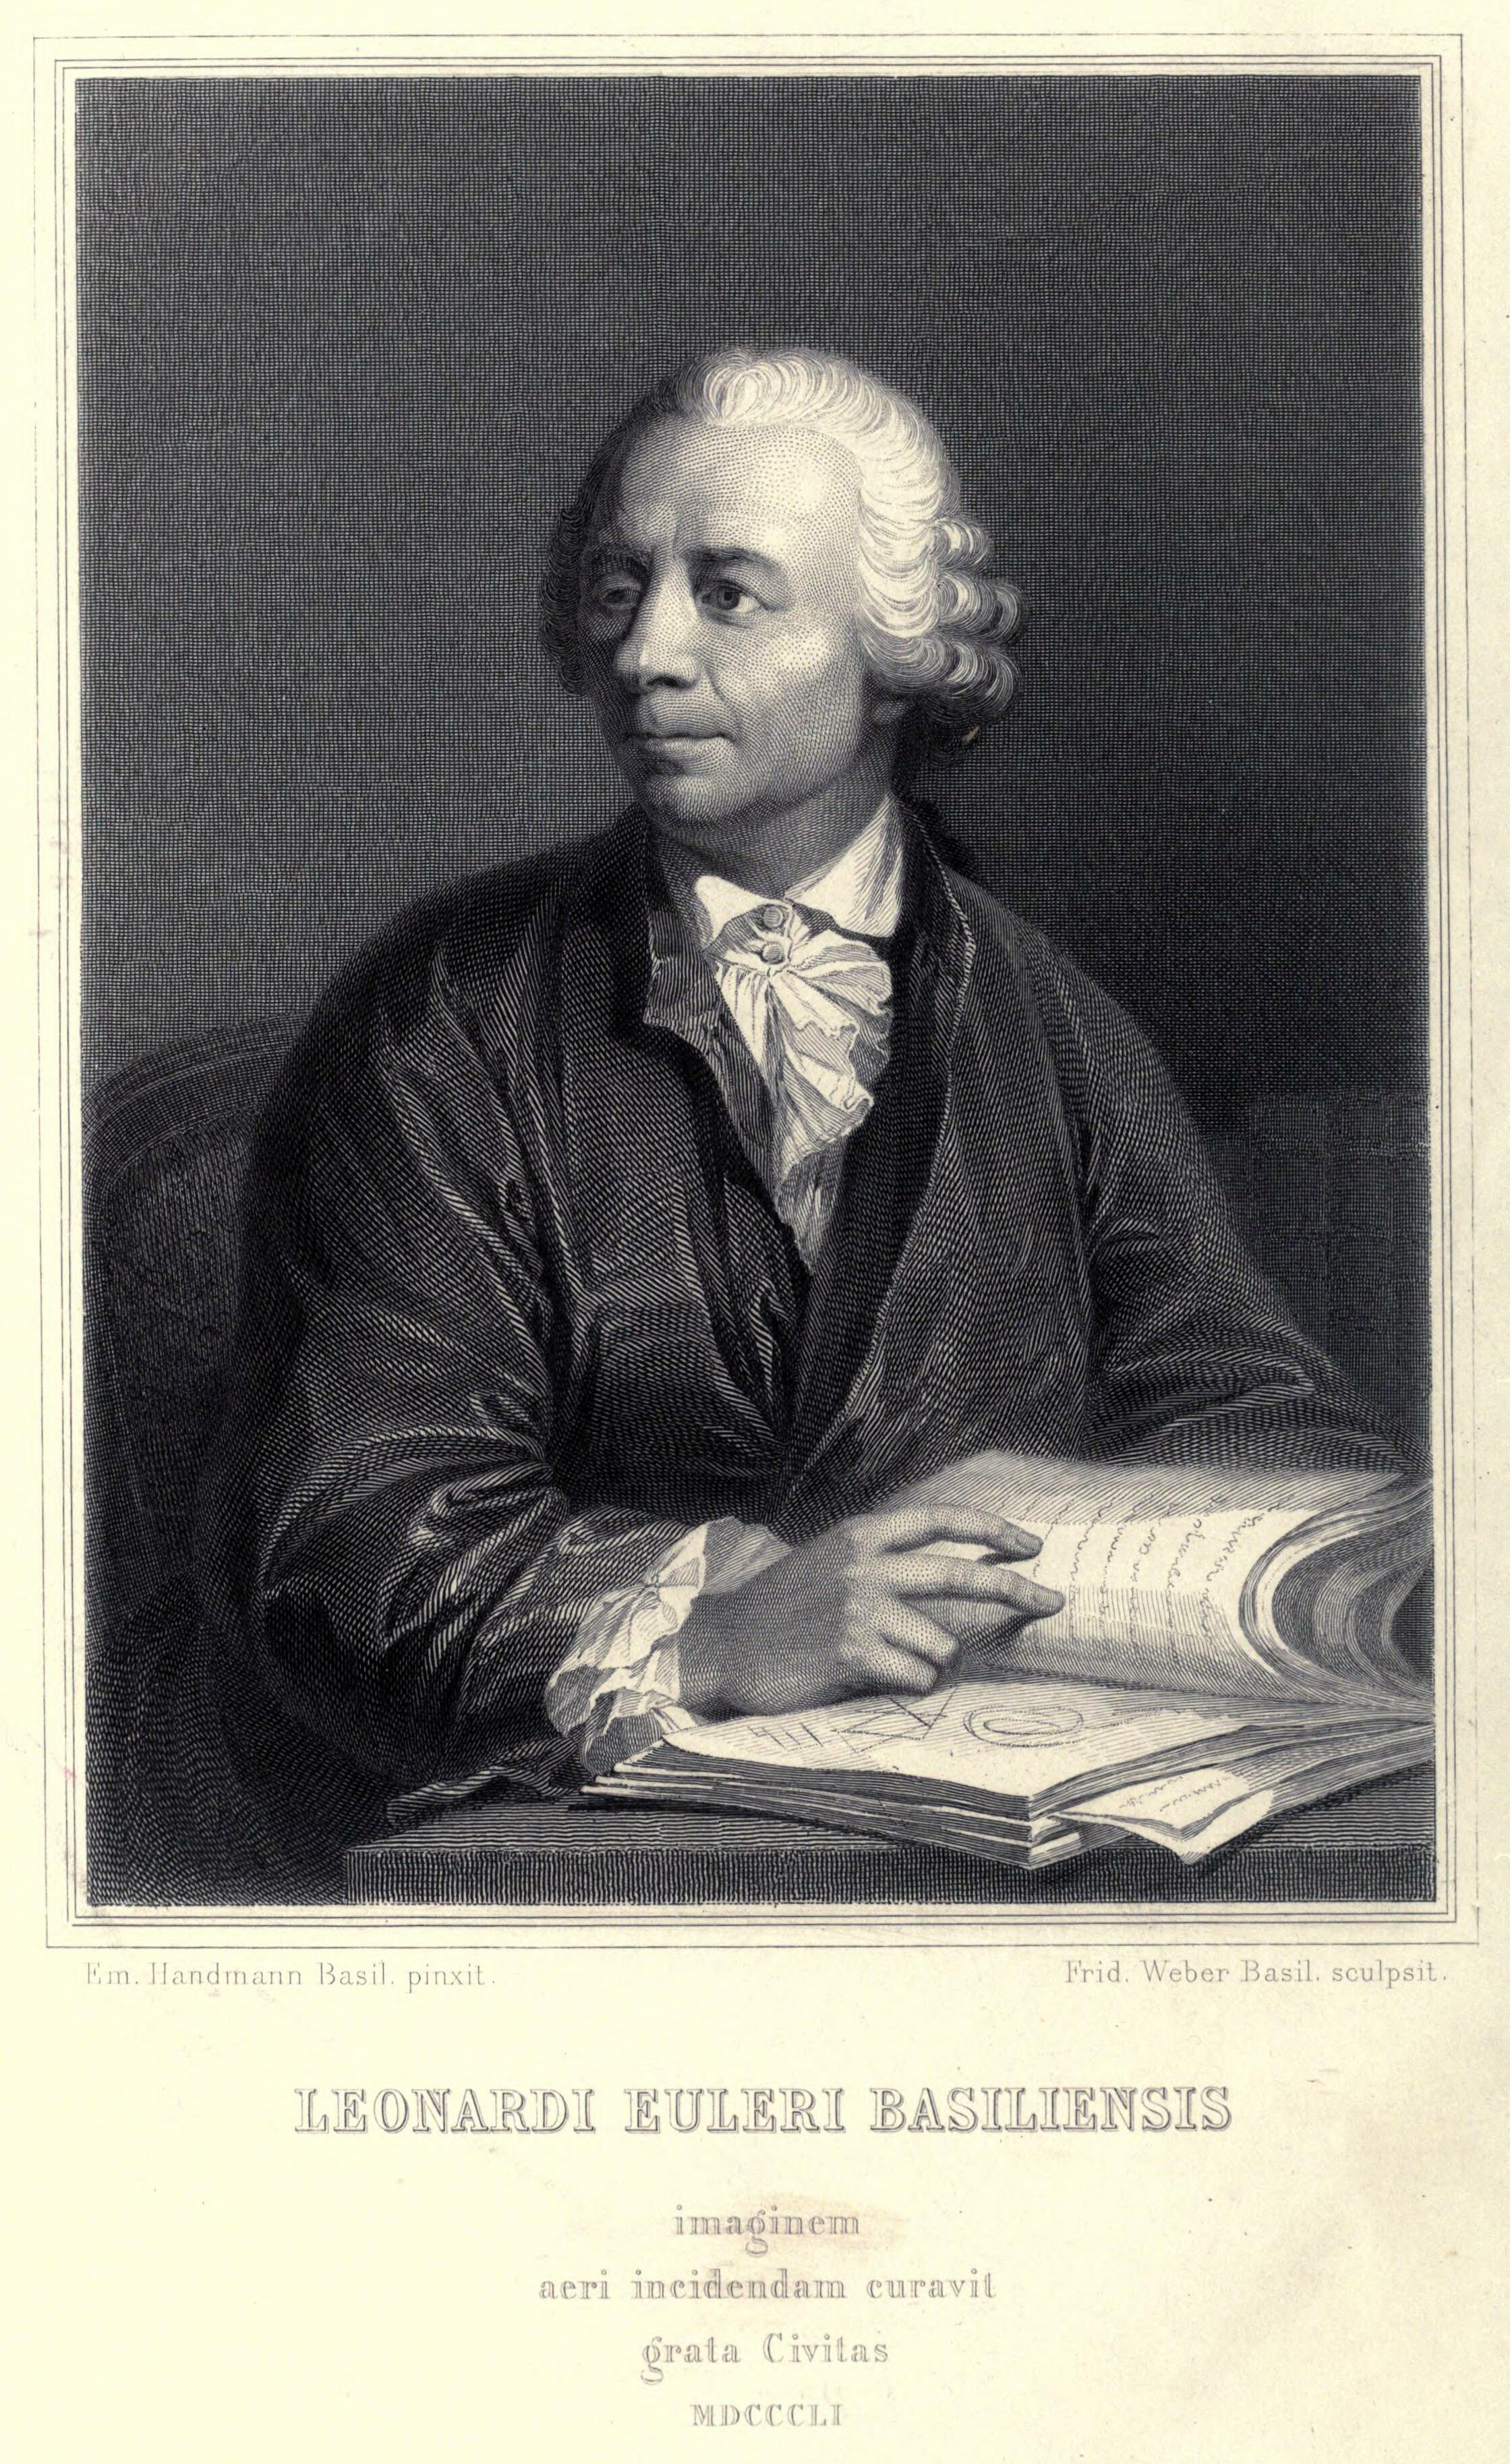
\includegraphics[
        alt={Portrait of Leonhard Euler.},
        height=\dimexpr.95\textheight-2pt\relax
      ]
      {figures/Euler.jpg}%
    };
  \end{tikzpicture}
  \caption[Leonhard Euler]{Leonhard Euler. Engraving by Friedrich Weber.}
  \label{figure:euler}
\end{figure}
While Fermat laid the groundwork for modern number theory, we should mention that the concept of \emph{function} hasn't been crystallized until Leibniz coined the term in 1673, using it to describe quantities related to curves, such as slopes, tangents, and areas. Bernoulli played a significant role in expanding the idea of functions.
He used the term explicitly in 1718, describing it as a quantity dependent on another variable. Euler provided the first modern definition of a function in his \textsc{Introductio in Analysin Infinitorum} (1748) \cite{euler1988}.
He emphasized that functions could include both algebraic (e.g., polynomials) and transcendental forms (e.g., trigonometric and exponential functions). Peter Gustav Lejeune Dirichlet was the first to define functions abstractly as a correspondence between two sets, removing the requirement for expressions or formulas.
This abstraction was a key insight for the theorem that we now know as \emph{Dirichlet's theorem}: Every arithmetic progression
\begin{equation*}
  a,\ a+b,\ a+2b,\ a+3b,\ \ldots
\end{equation*}
in which $a$ and $b$ are coprime, contains an infinitude of primes. Dirichlet proved his theorem in 1837, more than 150 years after Leibniz first coined the term of function.

Euler's Introductio in Analysin Infinitorum marked the beginning of \emph{analytical number theory}. As we mentioned before, Euler defined functions here and established the notation $f(x)$ of a function applied to its variable, which we still use today. He derived the famous formula for complex exponentials
\begin{equation*}
  e^{ix}=\cos(x) + i \sin(x).
\end{equation*}
This identity connects the exponential function, trigonometric functions, and the imaginary unit. The Riemann zeta function $\zeta(s)$ makes its first appearance here in a complex variable $s$, and he derived the celebrated \emph{product formula}
\begin{equation*}
  \zeta(s)=\sum_{n=1}^{\infty}\frac{1}{n^s}=\prod_{p\,\mathrm{prime}}\frac{1}{1-p^{-s}}.
\end{equation*}
More generally, Euler explored infinite series and products. The \emph{Basel summation formula}
\begin{equation*}
  \sum_{n=1}^\infty \frac{1}{n^2}=\frac{\pi^2}{6}
\end{equation*}
was first proven here, which was one of Euler's most celebrated achievements. Euler was keen to explore the connection between geometry and analysis, and in Introductio in Analysin Infinitorum, he advanced the idea that the study of functions and infinite series could provide new insights into geometric problems. He showed how techniques from analysis could be used to solve problems in geometry and vice versa, fostering the development of applied mathematics.

\subsection{Johannes Carl Friedrich Gauss}

\begin{figure}[p]
  \centering
  \begin{tikzpicture}
    \node[inner sep=0pt, rounded corners=0.5em, clip] {%
      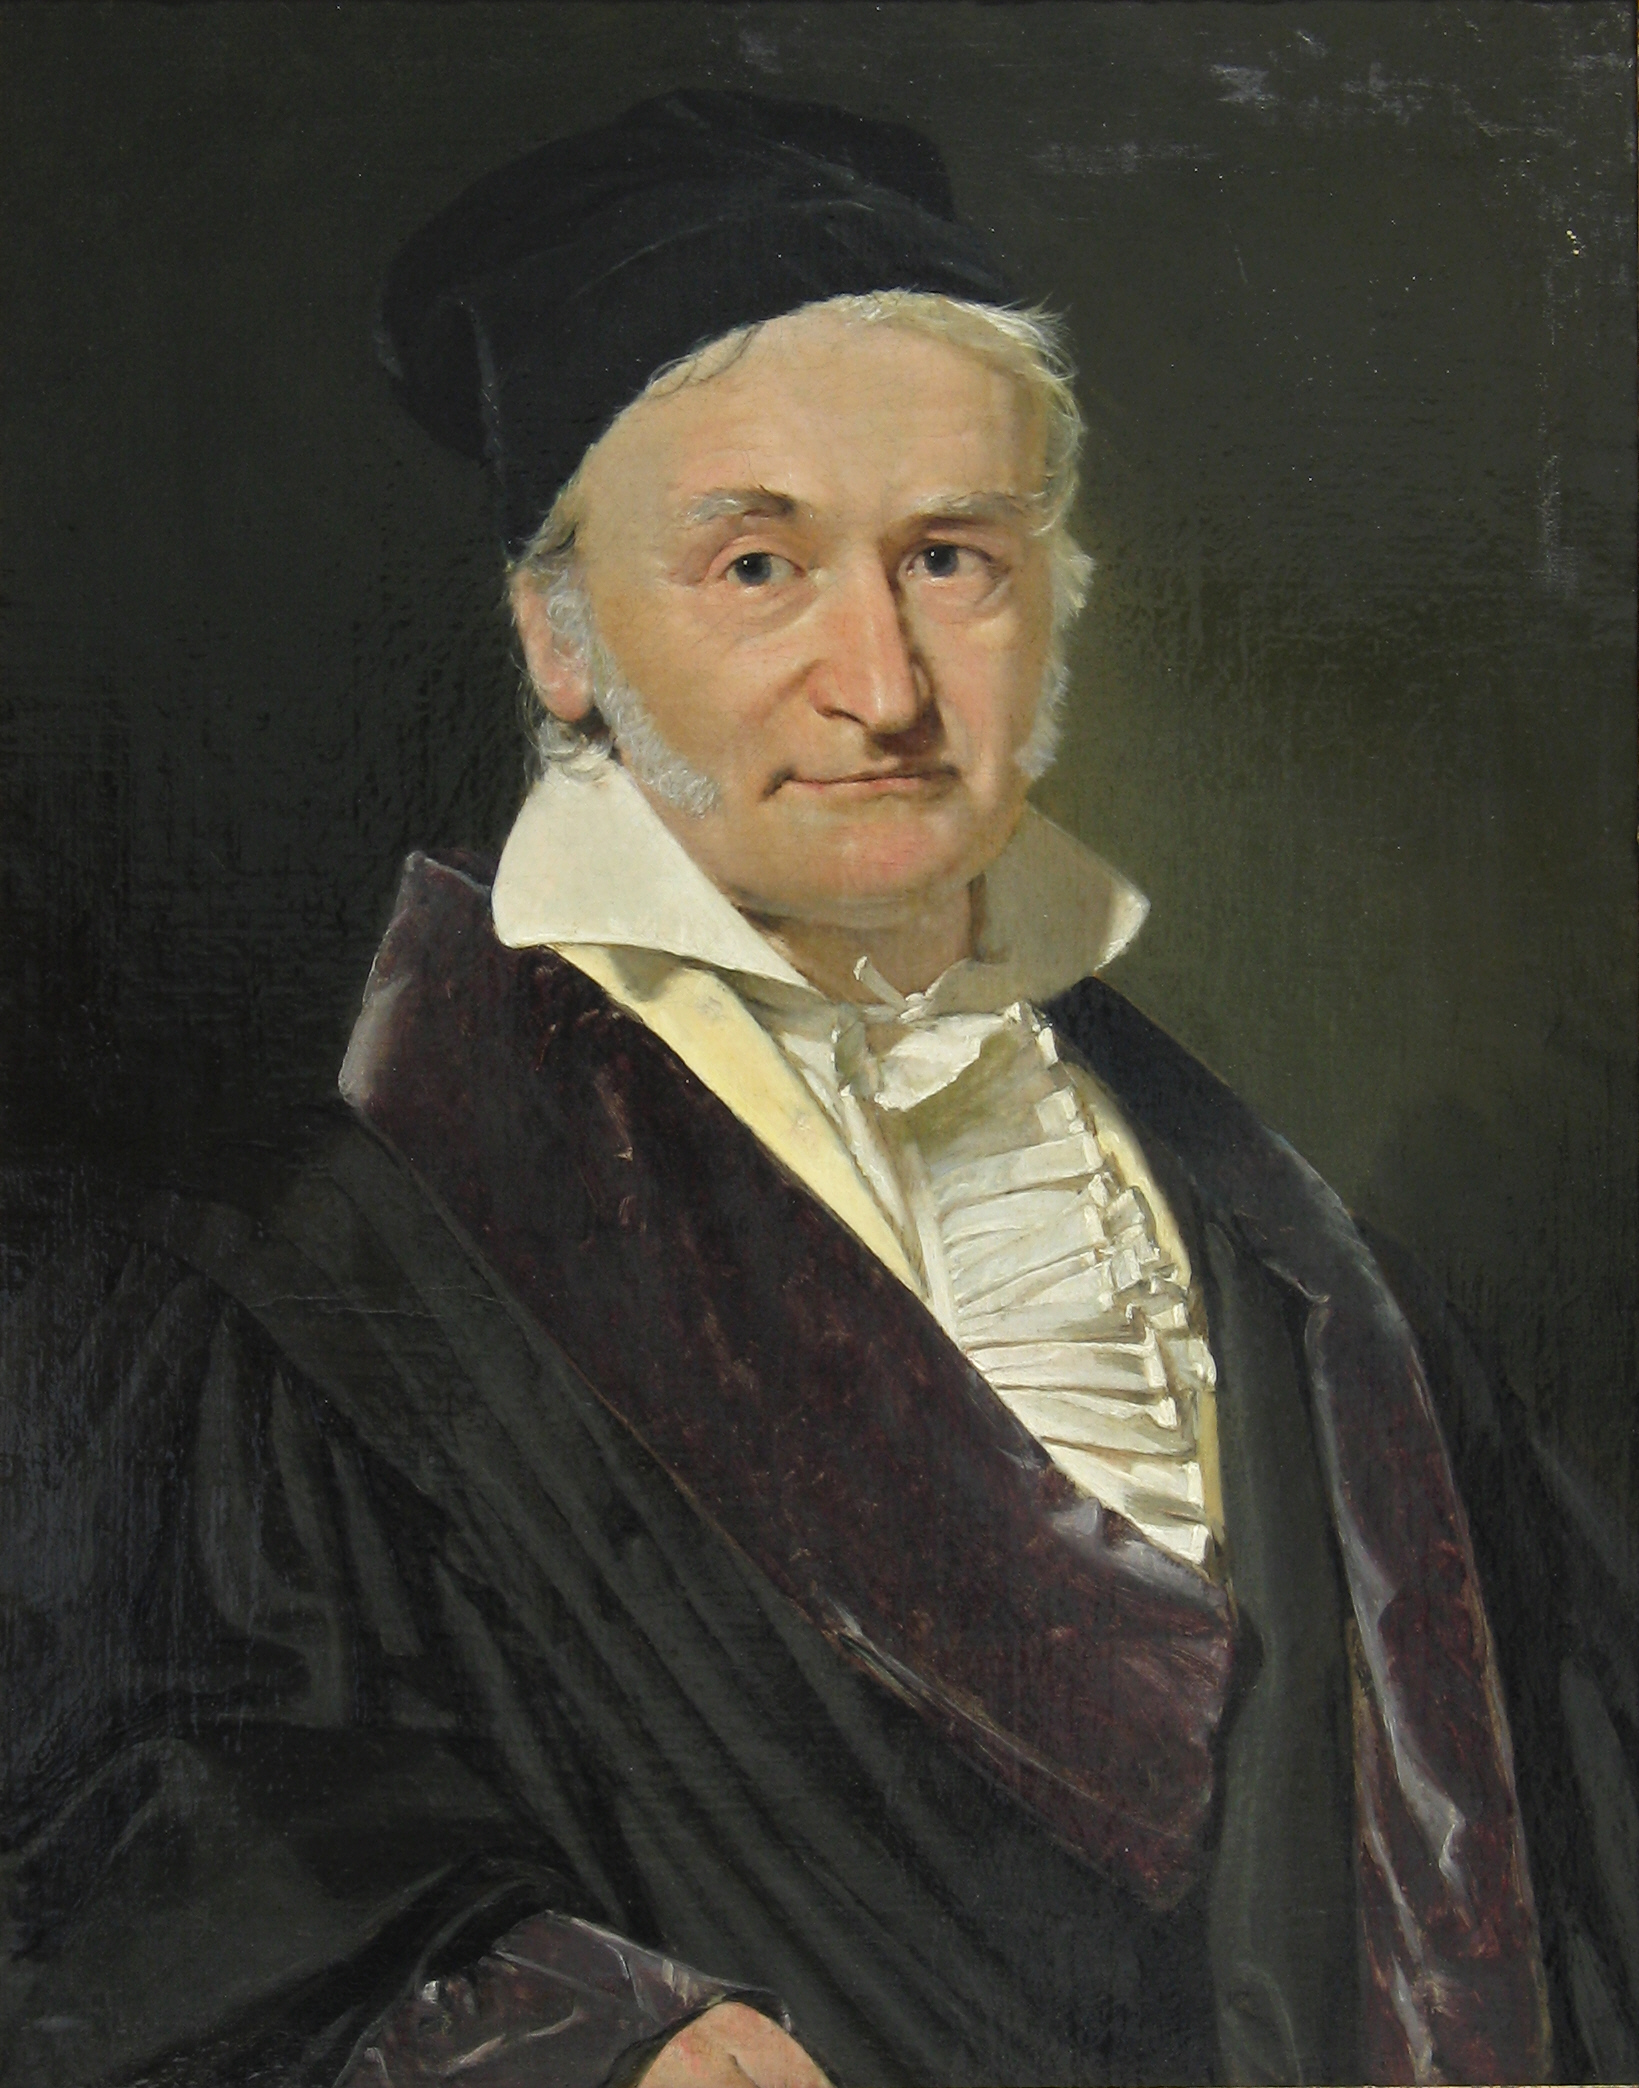
\includegraphics[
        alt={Portret of Carl Friedrich Gauss.},
        height=\dimexpr.95\textheight-2pt\relax
      ]
      {figures/Gauss.jpg}%
    };
  \end{tikzpicture}
  \caption[Carl Friedrich Gauss]{\sloppy{Carl Friedrich Gauss. Painting by Christian Albrecht Jensen.}}
  \label{figure:gauss}
\end{figure}
Building on the work of Euler, Gauss began using the properties of the zeta function and other analytic methods to investigate the distribution of the primes. His seminal work \textsc{Disquisitiones Arithmeticae} \cite{gauss1986} is often considered the starting point of the study of the distribution of primes, ultimately leading up to the \emph{Prime Number Theorem}. Gauss conjectured that the number $\pi(n)$ of primes below a number $n$ satisfies the asymptotic law
\begin{equation*}
  \pi(n)\sim\frac{n}{\log(n)}.
\end{equation*}
This conjecture was proved independently by Jacques Hadamard and Charles Jean de la Vallée Poussin. Furthermore, Gauss laid the foundation for modular arithmetic, and proved the celebrated law of quadratic reciprocity, which tells us when a quadratic equation modulo a prime number is solvable. More precisely, it states that if $q\equiv 1\pmod{4}$ then the congruence $x^2\equiv p \pmod{q}$ is solvable if and only if the congruence $x^2\equiv q\pmod{p}$ is solvable.

A brief remark on the interesting etymology of the word theorem is in order. The English word \emph{theorem} ultimately derives from the Ancient Greek {\greekfont θεώρημα} (the\={o}r\={e}ma), literally “that which is seen”, and by usage in classical philosophy as an “object of contemplation”. The verb {\greekfont θεωρεῖν} (\emph{theōreîn}, “to observe, examine”) and the agent noun {\greekfont θεωρός} (\emph{theōrós}, “spectator”) are close relatives, and ultimately give us both `theorem' and `theory'.

In Euclid's \textsc{Elements}, specifically through the careful editorial work and commentaries of the Byzantine scribes, we start seeing the label \emph{theōrēma} for statements that require deductive proof, in contrast to the “givens” ({\greekfont ὑπόθεσις}, hypóthesis) and “proof” ({\greekfont ἀπόδειξις}, apódeixis). However, the fixed label \emph{Theōrēma} for such statements emerges more clearly in Medieval translations into Late Latin and Middle French of the \textsc{Elements}, through the editorial adjustments made by his copyists. The Late Latin word \emph{theorema} and the Middle French word \emph{théorème} both retained the meaning “proposition that is to be proved”.

Euclid's \textsc{Elements} was first translated into English by Sir Henry Billingsley in 1570, who was mayor of London at the time, with a preface written by John Dee. This Billingsley--Dee edition of Euclid’s \textsc{Elements} established \emph{theorem} in the English language as a word meaning “proposition that is to be proved”. Over the ensuing centuries, the word theorem came to mean exclusively a mathematical assertion proven from axioms, definitions, and previously established theorems.

\subsection{Contemporary Mathematics}

So far, we have covered some of the most celebrated advances in humanity's understanding of numbers up to the early 19\supth{} century. Mathematics has made rapid progress since then. Bertrand's postulate, which asserts that there is always at least one prime $p$ between $n$ and $2n$, for any $n>1$, was proven by Pafnuty Chebyshev in 1852, and Ben Green and Terence Tau proved in 2004 that the sequence of prime numbers contains arbitrarily long arithmetic progressions.

The 20\supth{} century saw the emergence of the Langlands program, a far-reaching research program that aims to connect number theory, representation theory, and algebraic geometry. With the contributions of mathematicians like André Weil, Robert Langlands, and many others, the program has shaped much of the direction of modern research in number theory and its applications to other branches of mathematics.

Even today fundamental concepts such as sets and functions continue to evolve. We live in an era of digital computation, with tools far beyond the reach of Fermat, Euler, and Gauss, where essentially all recorded knowledge is readily available to almost anyone. This computational revolution has also given rise to powerful tools like proof assistants; that is, computer programs designed to construct and formally verify mathematical proofs. Since proof assistants are programming languages, they are often based on type theory rather than set theory, slightly changing the way mathematics is done. Functions in type theory are even more general than Leibniz, Euler, and Dirichlet envisioned: unlike in set theory where functions are a specific kind of relations between sets, functions in type theory are primitive entities satisfying certain rules for evaluation, and they have an extra dependency built in, allowing types of their outputs to depend on the input. Proof assistants are being used with great success to formally verify advanced mathematical theorems. Georges Gonthier formally verified the Four Color Theorem and the Odd Order Theorem, and Tom Hales verified Kepler's conjecture about sphere packings. A current effort led by Kevin Buzzard aims to formally verify Fermat's Last Theorem.

Today, number theory continues to be one of the most active and fruitful areas of mathematical research, all of which started simply with counting on ten fingers.

\section{The Concept of Number Through History}

Many people are familiar with numbers through everyday experiences like counting, measuring, or comparing quantities. From a young age, we develop an intuition about how numbers behave. Our experience with numbers reveals patterns and properties that seem to always be true. For example, we quickly learn that it does not matter in which order we add two numbers: Given two numbers $a$ and $b$ it is always true that $a+b=b+a$. Truths such as this one seem so self-evident that we might be tempted to just accept them. However, for a rigorous mathematical theory we need to be more careful. Mathematicians require proofs. Checking a property for every number up to a hundred, a million, or even $10^{27}$ might confirm a pattern, but infinitely many numbers remain beyond such finite checks. Mathematical proofs, on the other hand, are logical arguments that establish beyond any possibility of doubt why certain properties hold universally for all numbers, or at least for precisely defined sets of numbers. To reason about all natural numbers at once, we need formal principles that extend beyond empirical observation and anecdotal evidence. In order to discover such reasoning principles, we need to find out first what the natural numbers really are, a question with a rich and very interesting history.

% Clarify that Nicomachus lived around 100 CE, while Euclid lived around 300 BCE, implying that the transition used from the Pythagorean school of thought to Euclid's school of thought might not be historically accurate.

Although natural numbers arise from counting, the notion of number is not inherently linked to any particular collection of entities being counted. Scholars in the Pythagorean tradition were among the first to articulate this insight. Nicomachus emphasized in his \textsc{Introduction to Arithmetic} the concepts of \emph{monad} and \emph{dyad} for the totality of all things that come in one or two units \cite{nicomachus1926}. Nicomachus ascribed divine properties to the monad, or unity: ``{\itshape It generates itself without beginning, without end, and appears to be the cause of enduring, as God in the realm of physical actualities is in such manner perceived of as a preserving and guarding agent of nature}''. Nicomachus drew strong parallels between the monad and the concept of sameness, and dually between the dyad and the concept of otherness. He also emphasized that numbers were composed of monads. In other words, the monad is the source of all numbers. Although mathematicians do not ascribe divine properties to numbers anymore, we see here the emergence of some important ideas. The first is that all numbers are generated from the monad, that is, unity. The second idea is to connect unity with sameness. The idea that all things equal to a given object form a unit, or a singleton, anticipates a fundamental principle of equality. However, we shall forego the interesting digressions that we could make about equality and focus our attention on the concept of number.

Euclid takes a more abstract point of view, in which the concept of number is defined without relating it to the divine conception of the monad. For Euclid, a \emph{unit} is the conceptual principle by which an individual object is identified as one, and a \emph{number} is a multitude composed of such units in a discrete fashion \cite{euclid2015}. In other words, the concept of unit captures the notion of oneness, but this is distinct of the number $1$ itself. Both Nicomachus's and Euclid's views on the concept of number were highly influential throughout late antiquity and the Middle Ages, particularly through Boethius's Latin rendition of Nicomachus's \textsc{Introduction to Arithmetic} \cite{kaylorphillips2012} and Adelard of Bath's translation of Euclid's \textsc{Elements} \cite{clagett1953}.

While Pierre de Fermat is regarded the founder of modern number theory, he did not write extensively on the philosophy of mathematics. Nevertheless, certain themes in his correspondence and work show a clear orientation. For him, mathematics is about truths intrinsic to numbers. Numbers were the object of exact reasoning. He emphasized that \emph{induction}, by which mathematicians up to the early 19\supth{} century understood experimental verification, was insufficient to establish universal truths of numbers. Nowadays, this historical use of the word induction is sometimes called \emph{empirical induction}. Among Fermat's lasting contributions was his method of infinite descent, a method of proof by contradiction in which one shows that any supposed solution would lead to an ever-decreasing sequence of natural numbers, which is impossible.

With Euler, we witness a significant conceptual expansion. In his \textsc{Elements of Algebra}, Euler extended the notion of number beyond the natural and rational to encompass negative numbers, irrationals, complex numbers, and even infinite series. He was among the first to conjecture that constants like $e$ and $\pi$ are transcendental; that is, not the roots of any algebraic equation with rational coefficients. For Euler, numbers were entities governed by formal laws, irrespective of whether they corresponded to geometric magnitudes. Euler's broadening of the concept of numbers, and his use of analytic methods would eventually spark debates about the foundations of mathematics and the logical principles underlying mathematical truth.

In the 19\supth{} century, the nature of mathematics itself began to change. The emergence of non-Euclidean geometry was a challenge to the status of Euclid's Elements as the de facto foundation of mathematics, and Weierstrass's discovery of continuous, nowhere differentiable functions meant that one could not simply rely on intuition in the study of calculus and analytics. Furthermore, with Galois's use of symmetries in order to show that quintic equations had no solutions expressible in terms of radicals, abstract algebra became a prominent subject of mathematics with algebraic objects that have little in common with numbers except for a few formal laws. These discoveries underscored the need for a more solid foundation of mathematics, ultimately resulting in the emergence of Frege's logicism and set theory.

Nevertheless, the question of formally defining the set of natural numbers was left mostly unexplored until the second half of the 19\supth{} century. Even as late as 1886, Kronecker is quoted as proclaiming that ``God created the integers, all else is human work'' \cite{weber1893}, not helping the cause of finding a definition of the natural numbers. In \emph{Was sind und sollen die Zahlen?} (translated to English as \emph{What are numbers and what should they be?}), Dedekind was the first to formally define the set of natural numbers. His idea was that the number zero and the successor function together should be sufficient to describe all the natural numbers. He formalized this idea in 1888 by specifying that the set of natural numbers is a \emph{simply infinite set}, meaning that there is a one-to-one function $S:\mathbb{N}\to\mathbb{N}$ such that every element of $\mathbb{N}$ can be reached by iteratively applying $S$ to an element $0$, which is not itself a value of $S$ \cite{dedekind1888}. Dedekind showed furthermore that all simply infinite sets are similar to each other; in modern termimology, he showed that all simply infinite sets are \emph{isomorphic}. Thus, Dedekind's definition was structural in nature, in the sense that it captured the structure a set must possess in order for it to be considered a set of natural numbers.

Not much later, Giuseppe Peano arrives at a very similar definition of the set of natural numbers. In \textsc{Arithmetices principia nova methodo exposita} he established the set of natural numbers as a set satisfying a small number of axioms, the celebrated \emph{Peano axioms} \cite{peano1889}:
\begin{enumerate}
\item For any two natural numbers $x$ and $y$ we have
  \begin{equation*}
    (x=y)\Leftrightarrow (S(x)=S(y)).
  \end{equation*}
\item There is no natural number $x$ such that $S(x)=0$.
\item For any set $A$, if $0\in A$ and if for any natural number $x$ we have $(x\in A) \Rightarrow (S(x)\in A)$, then every natural number is in $A$.
\end{enumerate}
The first axiom establishes that the successor function $S$ is one-to-one. This means that every natural number is the successor of at most one natural number. The number $0$ itself is, in the setup of Dedekind and Peano, not a successor by the second axiom. The third axiom encodes \emph{mathematical induction}. The notation $x\in A$ means that $x$ is an element of $A$, or in other words that $A$ contains the element $x$. Thus, Peano's third axiom asserts that if $A$ is a set containing $0$ and containing the successor of every element it contains, then it contains all the natural numbers. While the similarity between Dedekind's and Peano's approach is clear, we note Dedekind's approach was structural, set-theoretic, and intended for a philosophical audience, Peano's approach was formal, logical, and symbolic.

A common alternative way of formulating mathematical induction is as follows. Given any property $P(n)$ expressing a condition of an arbitrary natural number $n$, in order to prove that $P(n)$ is true for all $n$ it suffices to prove that:
\begin{enumerate}
\item The property $P(0)$ is true.
\item For all $n$, if the property $P(n)$ holds then the property $P(n+1)$ holds.
\end{enumerate}
Mathematical induction formalizes the idea that every natural number is either $0$ or it is the successor of a previous natural number. Proving a property for all natural numbers therefore breaks down in two cases: The \define{base case} in which we prove that $P(0)$ is true, and the \define{inductive step} where we prove that $P(n+1)$ is true provided that $P(n)$ is true.

While proofs by mathematical induction go back to antiquity, the first to formulate the mathematical induction abstractly as a method of proof was Blaise Pascal in his \textsc{Traité du triangle arithmétique} \cite{pascal1665}. In this work, he studied the triangle of numbers now named after him. In a passage on the ratios of two horizontally adjacent binomial coefficients he wrote:
\begin{quote}
  {\itshape
    Quoy que cette proposition ait une infinité de cas, j'en donneray une démonstration bien courte, en supposant deux lemmes.
    
    Le 1.~qui est évident de soy-mesme, que cette proportion se rencontre dans la seconde base; car il est bien visible que φ est à σ comme 1 à 1.
    
    Le 2.~que si cette proportion se trouve dans une base quelconque, elle se trouvera nécessairement dans la base suivante.  
  }
\end{quote}
Notice, however, that Pascal did not yet use the term \emph{induction} for this method of proof. As we mentioned earlier, mathematicians of his time understood the word induction to refer to the empirical method of extrapolating patterns from finite data. Augustus De Morgan was the first to coin the term \emph{mathematical induction} in 1838, albeit somewhat incidentally \cite{cajori1918}. In his article on this topic in the \textsc{Penny Cyclopedia} he coined the term \emph{successive induction}, but he used the phrase \emph{mathematical induction} in a concluding remark \cite{demorgan1838}. Through the efforts of Dedekind and Peano, the induction principle has evolved from a method of proof to a defining principle for the set of natural numbers. 

By the turn of the 20\supth{} century, set theory, as pioneered by Georg Cantor and developed further by Richard Dedekind and others, was increasingly seen as a promising foundation for mathematics. However, the emergence of paradoxes around 1900 prompted efforts to axiomatize set theory. Beginning with Zermelo's axioms in 1908 and refined into the Zermelo--Fraenkel system in the 1920s, set theory gradually became the de facto foundational framework for modern mathematics. This raises the question whether the natural numbers can be defined within Zermelo--Fraenkel's set theory. Von Neumann gave an elegant set-theoretic definition of the natural numbers: The number $0$ was defined as the empty set $\varnothing$, the number $1$ was defined as the set $\{0\}$ containing the empty set, the number $2$ was defined as the set $\{0,1\}$, and so on:
\begin{equation*}
  0:=\varnothing,\qquad 1:=\{\varnothing\},\qquad 2:=\{\varnothing,\{\varnothing\}\}\qquad 3:=\{\varnothing,\{\varnothing\},\{\varnothing,\{\varnothing\}\}\},\qquad\ldots
\end{equation*}
However, Von Neumann's definition is not the only possible definition. One can also define
\begin{equation*}
  0:=\varnothing,\qquad 1=\{\varnothing\}, \qquad 2:=\{\{\varnothing\}\},\qquad 3 := \{\{\{\varnothing\}\}\},\qquad\ldots
\end{equation*}
These two definitions are clearly distinct, since $0\in 2$ is true in Von Neumann's definition but false in the latter definition. This raises the question, if Zermelo--Fraenkel set theory is to be the foundation of mathematics, then what is \emph{the} set of natural numbers? Paul Benacerraf argued in his famous essay \emph{What numbers could not be?} that the essence of the set of natural numbers is its structure, much like Dedekind had already argued almost a century before him \cite{benacerraf1965}.

While mathematicians often prefer to work with sets, computer scientists might prefer to work with types.  The distinction is merely that of the logical framework being used: Most mathematicians rely on the Zermelo--Fraenkel set theory, while computer scientist rely on programming languages that often have a type theory in its foundation. Theorem proving in computer programs called \emph{proof assistants} is rapidly becoming a more essential mathematical activity for students and researchers alike. However, many of the most popular proof assistants are based on type theory, in which collections of mathematical objects are called types.

Modern mathematics is increasingly formalized in computer programs called \emph{proof assistants}. There are many libraries of formalized mathematics in active current development, containing vast amounts of mathematics from a wide variety of mathematical subjects. However, the foundation of most such systems is not set-theoretic. Instead, many proof assistants use \emph{dependent type theory} as their foundational language, which was developed in the 1970s and 80s by Per Martin-L\"of. Both sets and types are collections of abstract objects often referred to as \define{elements}, but the formalisms by which they are studied are different in character, thus justifying the different names \emph{sets} and \emph{types}. The way the natural numbers are introduced in type theory is also slightly different. Whereas the induction principles of Dedekind and Peano establish the inclusion of the set of natural numbers into other sets, the natural numbers in type theory come equipped with a \emph{structural induction principle} that allows one to define functions out of the natural numbers. Similar to the previous definitions, the type of natural numbers comes equipped with $0$ and a successor function. The structural induction principle states that in order to define a function $f(n)$ taking as input a natural number $n$ and as output an element of a set $A_n$, possibly depending on $n$, one has to specify:
\begin{enumerate}
\item an element $a_0\in A_0$, and
\item a function $h_n: A_n\to A_{n+1}$ for every natural number $n$.
\end{enumerate}
The function $f$ obtained in this manner satisfies the equations
\begin{align*}
  f(0) & = a_0, \\
  f(n+1) & = h_n(f(n)).
\end{align*}
From a type-theoretic perspective, there is no need to assume that the successor function is a one-to-one function or that $0$ is not a successor. Indeed, these two axioms can be derived from structural induction.

We have thus seen that the concept of number has evolved over thousands of years of mathematical effort and underwent refinements up to the second half of the 20\supth{} century. We will follow the type-theoretic approach, and take a structural approach to the subject. Thus, the set of natural numbers contains an element $0$ and a successor function, and together they generate all the natural numbers in the sense that functions out of the natural numbers can be uniquely specified with recursive definitions. Similarly, we will give in this course structural accounts of the set $\mathbb{Z}$ of all integers, and the set $\mathbb{Q}$ of rational numbers. In the remainder of this chapter, we will explore from a practical perspective what induction and recursion mean, and how to use them.

\section{Mathematical Language}


%%% Local Variables:
%%% mode: latex
%%% TeX-master: "number-theory"
%%% TeX-engine: luatex
%%% End:
